\section{Searchable Encryption}

\label{sec_state_se}

%- Problemstellung: wie herausfinden, ob für ein Datum bereits ein Pseudonym vorliegt, obwohl die Daten lediglich nicht entschlüsselbar vorliegen? Außerdem auch Notwendigkeit des  Nicht-Determinismus für Searchable Encryption erwähnen (Public Key Verfahren).
%
%- Lösungsmöglichkeiten aufbauend jeweils mit Bewertung der Möglichkeit:
%  - Entschlüsseln und überprüfen: nicht möglich durch threshold, außerdem performance
%  - Local Mapping
%  - Einfacher Hash: Bruteforce bei kleinem Werteraum einfach (bspw. Mitarbeiternamen)
%  - Searchable Encryption (siehe Grundlagen)
%    - MAC als einfachste Form deterministischer Verschlüsselung
%    - Andere Formen...
%    
%- Mögliche Bewertungskriterien:
%  - Was muss abgesichert werden und wo muss es vorliegen?
%  - Mehrere Suchworte zu einem Pseudonym möglich? (zB Name, IP, ... ) Gewünscht? Welche Vorteile könnte dies beispielsweise bezogen auf den Anwendungsfall der Insidererkennung bringen?
%  - Verteilte Pseudonymhaltung möglich? Was müsste verteilt werden?

Trifft ein neues Datum in dem System ein und soll pseudonymisiert werden, so muss überprüft werden, ob bereits ein Pseudonym für das Datum vergeben wurde. 
Da die Daten jedoch in  verschlüsselter Form vorliegen, stellt sich die Frage, wie diese Überprüfung erreicht werden kann. In Abbildung \ref{fig:se_overview} ist dieses Problem noch einmal anhand eines Beispiels dargestellt. Zu einem Zeitpunkt liegen in der Pseudonymtabelle Pseudonyme für zwei Benutzer \textit{User A} und \textit{User B} vor. Das diese Benutzer zu den Pseudonymen gehören, ist jedoch nicht offensichtlich, da die Daten verschlüsselt gespeichert sind. Sollen nun neue Logdaten verarbeitet werden, liegen zwei mögliche Fälle vor: 

\begin{itemize}
  \item Es liegt bereits ein Pseudonym für den Benutzer vor (linker Bereich in der Darstellung). Hier muss das bereits vergebene Pseudonym \textit{0x1301} verwendet werden.
  \item Es liegt noch kein Pseudonym für den Benutzer vor (rechter Bereich in der Darstellung). Nun wird ein neues Pseudonym \textit{0x805A} angelegt und verwendet werden.
\end{itemize}

Verschiedene Lösungmöglichkeiten inklusive ihrer Vor- und Nachteile für das Problem, wie nun trotz der Verschlüsselung der Daten dieses Verhalten erreicht werden kann, werden in diesem Abschnitt beleuchtet.

\begin{figure}[]
    \centering
        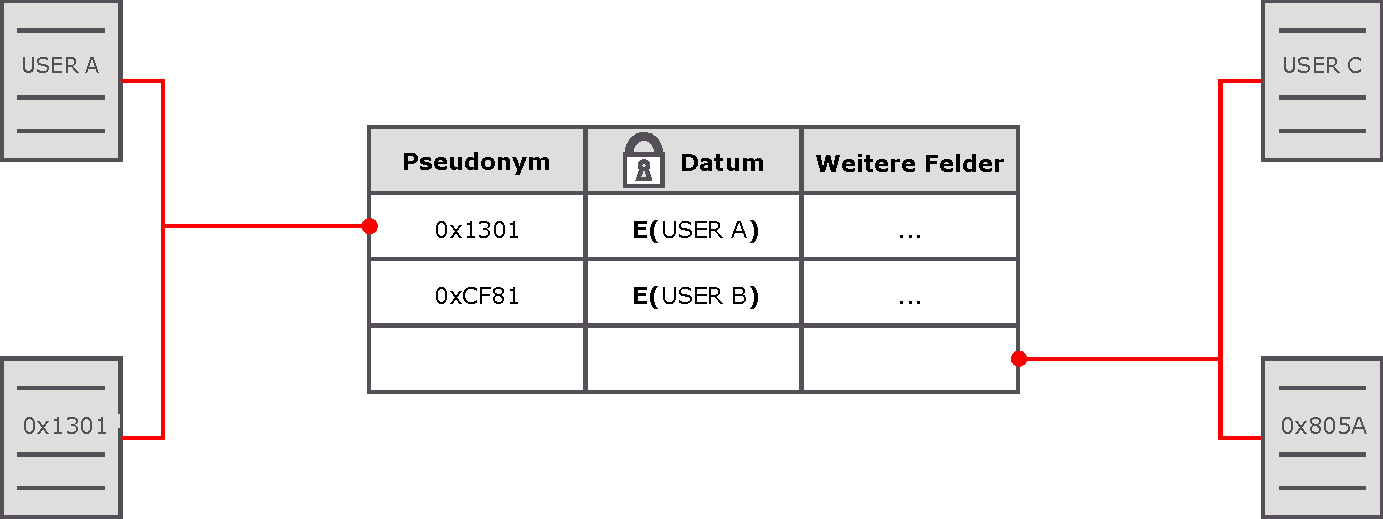
\includegraphics[width=0.9\textwidth]{dia/se_overview.pdf}
    \caption{Erhalt von Pseudonymen aus der Zuordnungstabelle: Links für den Fall eines bereits bekannten Datums (hier Benutzer), rechts für ein unbekanntes Datum.}
    \label{fig:se_overview}
\end{figure}

\subsection{Entschlüsseln aller Datensätze}

Da für die Verschlüsselung ein kryptographisches Schwellwertschema verwendet wird, scheiden zwei triviale Möglichkeiten aus: Das Entschlüsseln aller Datensätze zur Überprüfung wäre nicht nur unter Performance-Gesichtspunkten nicht wünschenswert. Es darf auch nicht möglich sein, da die \textit{Shares} zur Entschlüsselung nicht am Ort der Verschlüsselung vorliegen dürfen. Dies ist eine der Grundannahmen, die der Sicherheit des Systems zugrundeliegen. 

\subsection{Deterministische Verschlüsselung}
\label{sec_state_se_deterministic}

Die zweite ausscheidende Möglichkeit wäre das Überprüfen aller Einträge auf Schlüsseltextgleichheit. Bei Gleichheit eines Eintrages könnte das entsprechende Pseudonym zurückgeliefert werden. Hierzu müsste ein deterministisches Verschlüsselungsverfahren genutzt werden, das ein Datum immer auf den gleichen Schlüsseltext abbildet. Diese Möglichkeit scheidet jedoch aus, da es sich bei dem verwendeten Schwellwertschema um ein Public-Key-Verfahren, bei dem bei der Verschlüsselung ein Zufallswert einfließt -- folglich ein nicht-deterministisches Verfahren, handelt.\\
Dieser Nicht-Determinismus ist notwendig, da ansonsten zur Aufdeckung eines Pseudonyms auch ein Wörterbuchangriff mithilfe des öffentlichen Schlüssels des Schwellwertschemas genutzt werden könnte. Ein Angreifer würde alle möglichen Werte, die ein Datum annehmen kann, mit dem öffentlichen Schlüssel verschlüsseln und mit dem aufzudeckenden Eintrag vergleichen. Gleichheit der Schlüsseltexte würde den gesuchten Klartext liefern. Der im Kontext dieser Arbeit vorliegende kleine und bekannte Wertebereich (wie beispielsweise Mitarbeiternamen) würde diesen Angriff relativ effizient machen. Aus diesem Grund muss ein nicht-deterministisches Verschlüsselungsverfahren genutzt werden und damit ist die Überprüfung auf Schlüsseltextgleichheit nicht möglich.


\subsection{Nutzung von Hashfunktionen}

Ein weiterer Ansatz, der ebenfalls anfällig für diese Art von Wörterbuch-Angriff wäre, ist die Verwendung von (kryptographisch sicheren) Hashfunktionen zur Suche: Neben dem Pseudonym und dem verschlüsselten Datum wird ein Hash des Datums abgespeichert. Muss nun für ein neues Datum überprüft werden, ob bereits ein Pseudonym vorliegt, kann der Hash des Datums gebildet und mit allen vorliegenden Hashes verglichen werden. Bei Übereinstimmung wäre das Datum (mit großer Wahrscheinlichkeit) gleich dem verschlüsselten Datum und das Pseudonym könnte genutzt werden. Diese Möglichkeit ist jedoch durch den bereits erwähnten kleinen Wertebereich ebenso anfällig für einen Wörterbuchangriff: Ein Angreifer könnte mithilfe der bekannten Hashfunktion die Hashes aller Werte berechnen und mit dem des aufzudeckenden Pseudonyms vergleichen.

\subsection{Lokale Zuordnung}

Eine andere Möglichkeit ist die Anlage einer vor externem Zugriff geschützten Zuordungstabelle zwischen Datum und Pseudonym am Ort der Ersetzung. Bei Eintreffen eines neuen Datums kann in der Tabelle das zugehörige Pseudonym ermittelt werden oder falls es noch nicht existiert, ein neues Pseudonym erstellt und zusammen mit dem verschlüsselten Datum gespeichert werden. Diese Lösung wirda auch in \cite{goh2003} erwähnt.

Nachteil bezogen auf das für diese Arbeit zu entwickelnde System ist jedoch die notwendige Generierung von Pseudonymen und Speicherung der Zuordnungstabelle an der Stelle, an der neue Daten eintreffen. Hierdurch wird ein relativ leichtgewichtiger Proxy-Server wie er in der Architektur vorhergesehen ist (siehe Abschnitt \ref{sec_impl_architecture}) verhindert. Außerdem würde eine Kompromittierung dieser Komponente direkt zur Aufdeckung des Pseudonymzusammenhanges führen. \todo{Verhindert verteiltes System - diesen Aspekt betonen (mehrere Proxies, ...)}

\subsection{Message Authentication Codes}

\label{sec_state_se_mac}

Aufbauend auf der Hash-basierten Lösung lässt sich jedoch auch eine nicht für einen Wörterbuchangriff anfällige Lösung entwickeln. Dazu wird der verwendete Hash durch einen schlüsselabhängigen MAC (siehe Abschnitt \ref{sec_mac}) ersetzt. Beim Speichern eines neuen Eintrags wird dazu unter Zuhilfename eines zufällig generierten Schlüssels ein MAC über das Datum berechnet und mit dem Eintrag gespeichert. Für ein Datum kann jetzt durch Überprüfen aller MACs bestimmt werden, ob bereits ein Pseudonym vergeben wurde. Ein Angreifer kann den beschriebenen Wörterbuchangriff jedoch ohne Kenntnis des Schlüssels nicht ausführen.

Bei dieser Lösung handelt es sich um eine einfache Form der Searchable Symmetric Encryption wie sie in Abschnitt \ref{sec_basisc_se} dargestellt ist. Die durch Pseudonyme zu ersetzenden Daten bilden die zu durchsuchenden Dokumente. Der MAC bildet den Suchwort-Index für jeden verschlüsselten Eintrag und wird so auch als Trapdoor-Element für die Suche nach einem passenden Eintrag genutzt. Ausgehend von den Anforderungen des umzusetzenden Systems eignet sich dieser Ansatz: Er ermöglicht einer Komponente die Zuordnung eines Datums zu einem Pseudonym, ohne dass dass diese Zuordnung direkt gespeichert werden muss oder der Datenbank bei der Abfrage bekannt wird. Auch ein Wörterbuchangriff, der bei dem erwähnten kleinen Wertebereich geringen Aufwand bedeutete, wird verhindert. Aus diesen Gründen wird dieser Lösungsansatz in einem späteren Schritt im zu entwickelnden System umgesetzt.

Die Nutzung von deterministischer Verschlüsselung (mit der hier beschriebenen Verwendung eines MACs als Sonderfall) wird erstmals in \cite{bellare2007deterministic} beschrieben. Dort werden auch einige Schwächen dieser Lösung diskutiert: Die Datenbank erfährt durch den Suchindex bereits einiges über die gespeicherten Dokumente, da durch die deterministische Struktur gleiche Suchwörter auf gleiche Trapdoor-Elemente abgebildet werden. Diese Schwäche ist im Bezug auf den besonderen Anwendungsfall dieser Arbeit jedoch zu vernachlässigen, da Dokumente (meint Benutzernamen, ...) nur einmalig vorliegen dürfen. Eine weitere Schwäche, die auch in dieser Arbeit beachtet werden muss, ist, dass die Datenbank etwas über die Häufigkeit verschiedener Suchanfragen erfährt, da die Trapdoor-Elemente für ein bestimmtes Datum immer gleich sind. Durch Korrelation mit Hintergrundwissen könnte so möglicherweise in bestimmten Fällen der Inhaber eines Pseudonyms herausgefunden werden. 
\todo{Hash-Kollisionen und Geburtstags-Paradoxon hier erwähnen?}

\subsection{Weitere Möglichkeiten der Searchable Encryption}
\label{sec_state_se_furtherpossibilities}

%- SongWagner \cite{song2000practical}
%- survey \cite{wang2016}
%- goh \cite{goh2003}
%- chang \cite{chang2005}

Die im letzten Abschnitt betrachtete MAC-basierte Lösung funktioniert für den in dieser Arbeit behandelten Anwendungsfall. Bei der Abbildung Pseudonym zu Datum (wie den Benutzername) handelt es sich um eine 1:1-Abbildung, die lediglich von einer Komponente -- dem zu entwickelnden Log-Proxy -- abgefragt wird. 

In anderen Umgebungen bzw. Erweiterungen des in dieser Arbeit betrachteten Anwendungsfalls kann es jedoch auch andere Anforderungen geben. Vorstellbar wäre beispielsweise die verteilte Abfrage der Datenbank nach existierenden Pseudonymen. Für den MAC-basierten Ansatz müsste dazu zumindest der genutzte Schlüssel verteilt werden, was Kommunikation innerhalb der verteilten abfragenden Komponenten erfordert. Zusätzlich müssten auch die Sicherheitsauswirkungen dieser Lösung betrachtet werden.\\
Eine andere Erweiterung könnte die Mehrfachverwendung von Pseudonymen für verschiedene Merkmale eines Benutzers (Name, IP-Adresse, Signaturschlüssel, ...) sein, um die Erkennung von Insiderangriffen zu verbessern. Auch diese Erweiterung wäre mit dem MAC-basierten Ansatz nicht direkt abbildbar.

Andere Lösungsansätze für die in diesen Fällen entstehenden Probleme könnten Forschungsergebnisse aus dem Bereich der \textit{Searchable Encryption} bieten. In \cite{song2000practical} wurde von den Autoren das erste Searchable-Symmetric-Encryption-Schema entwickelt (siehe auch Abschnitt \ref{sec_basisc_se}). Verbesserte Schemata folgten in \cite{goh2003} und \cite{chang2005}. Durch diese sind variable Dokumentenlängen mit beliebig vielen Suchwörtern möglich, die auch nachträglich erweiterbar sind. Für den Aspekt der verteilten Abfrage könnten die Ergebnisse aus \cite{boneh2004public} genutzt werden, in dem sich die Autoren mit der Suche in mit asymmetrischen Verfahren verschlüsselten Daten befassen.\\
Eine Übersicht über weitere Ergebnisse in diesem Bereich lässt sich in \cite{wang2016} finden.